\chapter{Wprowadzenie do tematyki pracy, wykorzystane narzędzia}
%Ten rozdział mi nie gra jakoś, narzędzia są okej ale reszta mi nie pasuje
\section{Technologia VR}
Technologia rzeczywistości wirtualnej polega na tworzeniu w pełni sztucznego otoczenia, które wywołuje poczucie przebywania w zupełnie innym miejscu lub świecie. Dzięki specjalistycznym urządzeniom, takim jak gogle czy kontrolery ruchu, możliwe staje się obserwowanie i oddziaływanie na generowane wirtualnie obiekty w czasie rzeczywistym. Rozwiązania z zakresu VR wykorzystują zaawansowane techniki renderowania grafiki, precyzyjnie śledzą ruch głowy i dłoni, a także uwzględniają dźwięk przestrzenny, co pozwala na osiągnięcie wysokiego stopnia imersji. Technologia ta znajduje zastosowanie nie tylko w obszarze gier i rozrywki, lecz również w szkoleniach branżowych, symulacjach medycznych \ref{vr_example} i architektonicznych oraz w przemyśle, gdzie służy do prototypowania i prezentacji projektów. Wirtualna rzeczywistość sprzyja ograniczaniu kosztów wdrożeń oraz podnoszeniu efektywności procesów nauki i projektowania, ponieważ umożliwia wielokrotne testowanie różnych scenariuszy w ściśle kontrolowanym środowisku.

\begin{figure}[!htb]
    \centering
    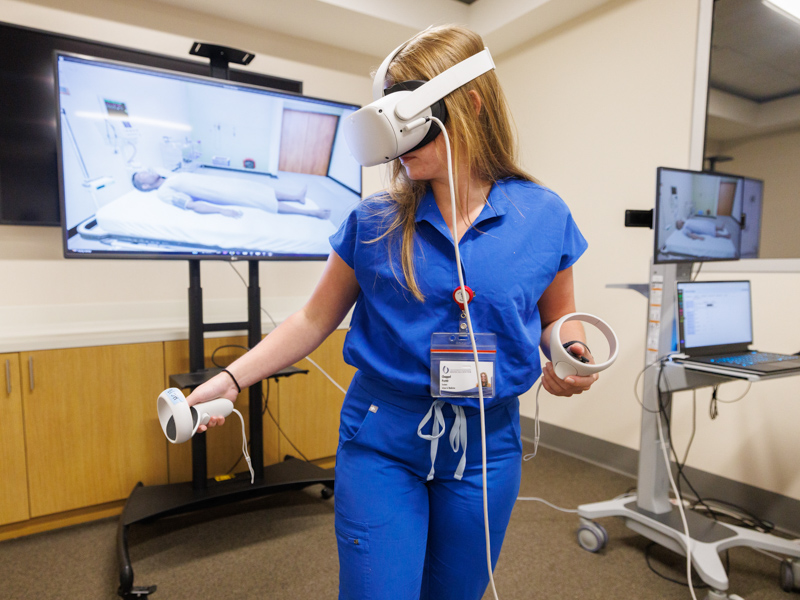
\includegraphics[width=0.8\textwidth]{images/vr_example.jpg}
    \caption{Symulator medyczny służący do szkolenia lekarzy}
    \label{vr_example}
\end{figure}\textbf{}

Tryby interakcji z VR
Siedzący (Seated VR)najczęściej stosowany w symulatorach lotniczych i wyścigowych, które wymagają precyzyjnego sterowania; stojący zwany rownież stacjonarnym
Stacjonarny 
Swobodny ruch (Room-scale VR)

Tryby renderowania i wyświetlania VR

Tryby śledzenia ruchu użytkownika

 Tryby użytkowania w zależności od platformy

 Tryby użytkowania VR według zastosowania

Czym jest Interfejs uzytkownika w VR

Czym są interakcje i jakie wyroznia sie metody interakcji w vr


 \section{Znaczenie UX w procesie projektowania}
 
 %W sytuacji, gdy użytkownik napotyka trudności w interakcji z przedmiotem, takim jak drzwi, i nie wie, jak wykonać określoną czynność (np. otworzyć drzwi), problemem nie jest sam użytkownik, lecz projekt produktu(Norman, 2013).



\section {Narzędzia i środowisko pracy}


 projektowania tej pracy był wybór odpowiednich narzędzi umożliwiających prototypownie, implementację oraz testowanie interfejsu w środowisku VR. Wybór używanej technologii jest kluczowy, aby zapewnić wysoką jakość doświadczeń użytkownika oraz zachować efektywność samego procesu projektowania.

\subsection{Figma}
Figma to podstawowe narzędzie służące do projektowania interfejsów użytkownika, jednocześnie umożliwia tworzenie interaktywnych klikalnych prototypów aplikacji. Jest to aktualnie jedno z najbardziej popularnych i bezpłatnych narzędzi w branży UX/UI. W projekcie Figma zostanie wykorzystana do stworzenia wstępnych projektów i prototypów interfejsów, a następnie do przetestowania rożnych układów elementów interfejsu. 
%(tu będzie dokumentacja figmy)
\subsection{Unity}
\textit{Unity} to jeden z najpopularniejszych wieloplatformowych silników do tworzenia gier wideo oraz interaktywnych aplikacji. Umożliwia zaawansowaną obsługę grafiki i fizyki, a w samym edytorze udostępniono rozbudowany zestaw narzędzi do projektowania scen, animacji i efektów graficznych \ref{unity_engine_example}. Proces programowania odbywa się przy użyciu języka \textit{C\#}.

W Unity dodano również wsparcie dla wirtualnej oraz rozszerzonej rzeczywistości, co przekłada się na szerokie zastosowanie tej technologii w szkoleniach, symulacjach czy działaniach marketingowych. Oprócz możliwości tworzenia zaawansowanych pod względem wizualnym scen, istotna jest też opcja łatwej integracji gotowych wtyczek obsługujących urządzenia AR i VR od różnych producentów. Rozbudowany system oświetlenia oraz post-processingu zapewnia szeroki wachlarz opcji i umożliwia dostosowanie grafiki pod dedykowane urządzenia, dzięki czemu można uzyskać zadowalającą jakość i odpowiednią optymalizację na urządzenia mobilne oraz wysoce realistyczną grafikę na komputerach osobistych.

\begin{figure}[!htb]
    \centering
    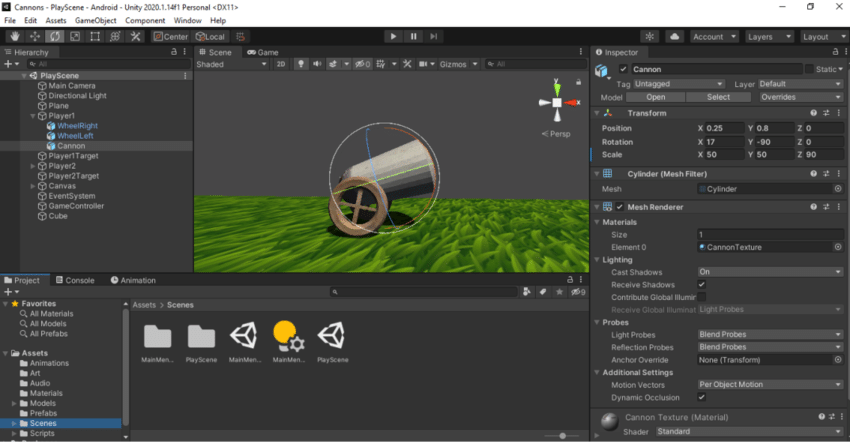
\includegraphics[width=0.8\textwidth]{images/unity.png}
    \caption{Przykładowy wygląd edytora Unity}
    \label{unity_engine_example}
\end{figure}

Regularne aktualizacje silnika rozszerzają jego funkcjonalność i dodają nowe rozwiązania, takie jak obsługa ray tracingu, DLSS oraz nowe narzędzia. Stały rozwój sprawia, że Unity zachowuje elastyczność w obliczu zmieniających się potrzeb rynku, a jego wszechstronność umożliwia realizację nawet najbardziej rozbudowanych koncepcji interaktywnych.

Społeczność skupiona wokół tego silnika udostępnia liczne materiały edukacyjne w postaci kursów i filmów, co znacząco obniża poziom wejścia, przyspiesza naukę oraz ułatwia rozwiązywanie ewentualnych problemów technicznych. Dokumentacja silnika jest regularnie rozwijana, a oficjalny sklep \textit{Asset Store} zapewnia dostęp do bardzo dużej ilości bezpłatnych oraz płatnych pakietów, obejmujących zasoby takie jak modele, tekstury i dźwięki oraz dodatkowe użyteczne narzędzia wraz z całymi gotowymi systemami ułatwiającymi stworzenie projektu i pozwalającymi ograniczyć koszty produkcji.


\subsection{Gogle VR}
Gogle VR to urządzenia, które całkowicie zasłaniają pole widzenia i wyświetlają przez użytkownikiem dwa identyczne, ale nieco przesunięte od siebie obrazy, które nałożone na siebie przez mózg dają wrażenie głębi. Wewnątrz gogli umieszczone są specjalne czujniki takie jak żyroskop, kamery i inne śledzące położenie i ruch głowy w przestrzeni. Dzięki temu użytkownik obracając głową faktycznie rozgląda się w przestrzeni wirtualnej obracając kamerą gracza.

Oprócz gogli istotne są również specjalne kontrolery zakładane na dłonie. Dzięki nim możliwa jest interakcja z wirtualnym otoczeniem, a specjalne czujniki i przyciski wykrywają pozycje palców i pozwalają określić, czy gracz w tej chwili próbuje złapać przedmiot. Całość wraz z systemem śledzenia pozycji dłoni pozwala dowolnie sięgać w różnych kierunkach, co pozwala mieć wpływ na obiekty w aplikacji. Gracz może na przykład chwycić przedmiot i rzucić nim, co pozwoli wywołać kolejne symulacje w fizyce.

Oprócz tego istnieje wiele różnych dodatków rozszerzających możliwości wirtualnej rzeczywistości, jak specjalne kombinezony monitorujących ruch oraz umożliwiających odczuwanie na skórze poprzez elektrostymulację nerwów i mięśni lub kapsuły, w których użytkownik ma możliwość skakania oraz poruszania się w dowolny sposób bez ryzyka, że uszkodzi coś w pokoju.

\subsection{Google Forms i inne narzędzia do analizy UX/UI}










%\section{Ogólne zasady projektowania interfejsów użytkownika}